\documentclass[a4,10pt]{article}
\usepackage[margin=0.85in]{geometry}
\usepackage{natbib}
\usepackage{times}
\usepackage{titlesec}
\usepackage{hyperref}
\hypersetup{
    colorlinks=true,
    urlcolor=blue,      % Makes \href and URLs blue
    linkcolor=black,    
    citecolor=black,    
    filecolor=magenta}

% Paragraph formating
\setlength{\parindent}{0pt}
\setlength{\parskip}{6pt}

% Modify spacing for section titles
\titlespacing*{\section}
{0pt}        % left margin
{8pt}       % space before (vertical)
{6pt}        % space after (vertical)

% Set document language and ensure correct language-specific typography
	\usepackage{polyglossia}
	\setmainlanguage[variant=british]{english}
	\usepackage[british]{selnolig}
	

%% Load packages for correct mathematical typesetting
	\usepackage{amsmath} 
	\usepackage{amssymb} % loads amsfonts, allowing mathfrak and mathbb
%	\usepackage{xparse}\usepackage{physics} % adds loads of useful cmds
	\usepackage[output-decimal-marker={.},
				exponent-product = {\cdot}, 
				range-units=single,
				range-phrase={–},
%				detect-mode, 
				]{siunitx} 	% Correct typesetting of units
    \usepackage[math-style=TeX,
                bold-style=ISO,
                nabla=upright,
                partial=upright
                ]{unicode-math} 
\newcommand{\pdv}[2]{\ensuremath{\frac{\partial #1}{\partial #2}}}
\newcommand{\mbeq}{\overset{!}{=}}

%% Utility packages
%	\usepackage[hyphens]{url}
%	\usepackage{enumerate}

%\usepackage[backend=biber,style=ext-authoryear-comp, maxnames=2]{biblatex}
%    \DeclareLanguageMapping{english}{british}
%    \DeclareNameAlias{sortname}{family-given}
%	\renewcommand{\mkbibnamefamily}[1]{\textsc{#1}} 
%	\renewcommand{\mkbibnameprefix}[1]{\textsc{#1}}
%    \renewcommand{\finalnamedelim}{\space\&\space}
%	\renewcommand{\multicitedelim}{;\space}
%	\renewcommand{\intitlepunct}{\space} % goes from « in: » to « in »
%\addbibresource{bibliography.bib}
%\usepackage[numbib,notlof,notlot,nottoc]{tocbibind}
\usepackage{blindtext}


\usepackage{graphicx}
\graphicspath{{figures/}}
%	\usepackage{wrapfig}
	\usepackage{float}
	\usepackage[font=small,justification=centerlast]{caption,subcaption}
 \usepackage{booktabs}
 \usepackage{multirow}
 \usepackage{comment}
\usepackage[table]{xcolor}
\usepackage{threeparttable}

%Last
%\usepackage[hidelinks, bookmarks]{hyperref} % hyperlinks!
%\hypersetup{
%    colorlinks=true,
%    urlcolor=blue,      % Makes \href and URLs blue
%    linkcolor=black,    
%    citecolor=black,    
%    filecolor=magenta}
\usepackage{cleveref} % clever section referencing; use \cref and \Cref


\usepackage{mathtools} % Better than amsmath alone

\usepackage[minimal]{yhmath}




\title{Forecasting the ECB Deposit Facility Rate -- An Iterative Taylor Rule Approach}
\author{Jonas Bruno, Marcos Constantinou, Benoit Goye}

\begin{document}

\maketitle

\begin{abstract}
We developed a comprehensive forecasting framework to evaluate various specifications of the Taylor Rule for the ECB Deposit Facility Rate. Our results indicate that a model incorporating an Auto-ARIMA process to forecast inflation and the output gap, augmented with lagged inflation outperforms all alternative specifications. We find that models excluding lag structures or those utilizing a shadow rate to quantify monetary policy at the Zero Lower Bound (ZLB) yield inferior predictive accuracy and higher utility loss.

\end{abstract}

\begin{figure}[b]
    \centering
    University of Lausanne -- Faculty of Business and Economics
    
    \noindent MScE Economic Forecasting for Decision Making 

\end{figure}


\newpage

\tableofcontents
\listoftables
\listoffigures


\newpage


\clearpage
\section{Introduction}\label{sec:intro}
\par The conduct of monetary policy by central banks relies fundamentally on the ability to forecast key macroeconomic variables and communicate policy intentions to market participants. In the European context, the European Central Bank's (ECB) deposit facility rate serves as the primary instrument for steering monetary policy in the euro area. Accurate forecasting of policy rates is crucial not only for central bank decision-making but also for financial market participants, governments, and businesses that must anticipate future monetary conditions to make informed decisions.
\par This paper develops and evaluates a forecasting methodology for the ECB deposit facility rate based on the Taylor rule framework. The Taylor rule, originally proposed by \cite{taylor1993discretion}, provides a systematic approach to understanding central bank behaviour by relating the policy interest rate to deviations of inflation from target and output from potential. Our methodology combines the theoretical foundation of the Taylor rule with time series forecasting techniques. Specifically, we employ ARIMA models to generate forecasts of the Taylor rule inputs—the inflation gap (deviation of HICP inflation from the ECB's 2\% target) and the output gap (estimated using the Hamilton filter applied to euro area real GDP), which are then combined to predict future policy rates. While we estimate specifications using both actual inflation and inflation expectations from the ECB Survey of Professional Forecasters, our primary results focus on models using actual inflation data. The forecasting challenge is particularly acute in the post-2008 financial crisis environment, which has been characterized by the zero lower bound (ZLB) constraint, unconventional monetary policies, and significant structural breaks. To address these challenges, we incorporate the Wu-Xia shadow rate \citep{wu2016measuring}, which captures the stance of monetary policy when conventional rates are constrained by the ZLB. We also employ rolling-window estimation techniques with a window size of 85 quarters (approximately 21 years) to account for time-varying relationships between policy rates and macroeconomic fundamentals.
\par We evaluate our forecasting methodology using quarterly data from 1999 Q1 to 2025 Q3 through a rigorous pseudo out-of-sample framework, conducting forecasts up to ten quarters ahead using a rolling window approach. The evaluation employs both absolute performance metrics (Mincer-Zarnowitz tests for bias and efficiency) and relative performance metrics comparing mean squared forecast errors against a benchmark ARIMA model using Diebold-Mariano tests. This comprehensive evaluation framework allows us to assess the practical utility of Taylor rule-based forecasts relative to atheoretical time series benchmarks. Our analysis reveals several key findings. First, we document significant structural breaks in the Taylor rule relationship, particularly around the onset of the ZLB period (2008 Q3) and the COVID-19 pandemic (2020 Q1), which motivate our use of rolling-window estimation. Second, we find that Taylor rule-based forecasts can provide competitive forecasting performance relative to benchmark ARIMA models, particularly at medium-to-long horizons. Third, we demonstrate that incorporating interest rate persistence through lagged dependent variables substantially improves forecast accuracy. Finally, we provide actual forecasts for the ECB deposit facility rate extending to 2028 Q1, accompanied by prediction intervals with uncertainty derived from the pseudo out-of-sample evaluation exercise.

\section{Literature Review}\label{sec:litreview}
\par The Taylor rule has become one of the most influential frameworks in monetary economics since its introduction by \cite{taylor1993discretion}. The original formulation proposed that the Federal Reserve's policy rate could be well approximated by a simple linear function of the inflation gap the deviation of actual inflation from the central bank's target and the output gap the percentage deviation of real GDP from potential GDP. The elegance and empirical success of this simple rule sparked an extensive literature examining its applicability across different countries, time periods, and policy regimes. \cite{clarida2000monetary} extended the Taylor rule framework by estimating forward-looking specifications for the Federal Reserve, Bundesbank, and Bank of Japan, demonstrating that central banks respond to expected rather than contemporaneous inflation. \cite{orphanides2001monetary} highlighted the importance of real-time data, showing that Taylor rule estimates can be substantially affected by data revisions and the mismeasurement of potential output. For the ECB specifically, \cite{gerdesmeier2004taylor} and \cite{fendel2009inflation} found that simple Taylor rules provide a reasonable description of ECB policy behaviour during the pre-crisis period, though with coefficients differing from Taylor's original calibration. \cite{gorter2008taylor} provided important evidence supporting the forward-looking nature of ECB policy, demonstrating that Taylor rules estimated using expectations data from Consensus Economics for inflation and output growth significantly outperform specifications based on realized outcomes, with the ECB taking expected inflation and expected output growth into account when setting interest rates. \cite{klose2023estimated} developed a comprehensive real-time database for the ECB decision dates with daily forecasts for inflation and output up to fourteen months ahead, finding that the ECB's inflation forecast horizon is rather long-term (over one year) while the picture for output is less clear, and demonstrating that these forecast horizons tend to be time-varying across different policy regimes.
\par The global financial crisis and subsequent period of extremely low interest rates posed significant challenges for both the implementation and estimation of Taylor rules. When policy rates are constrained by the ZLB, conventional Taylor rule estimates may fail to capture the true stance of monetary policy. \cite{wu2016measuring} addressed this issue by developing shadow rate models that estimate a hypothetical policy rate in the absence of the ZLB constraint. Their methodology, which we employ in this paper, provides a continuous measure of monetary policy stance throughout both conventional and unconventional policy regimes. \cite{krippner2013measuring} proposed an alternative framework based on a ``shadow short rate'' that uses a tractable approximation to model the term structure in ZLB environments, demonstrating its application to Japanese monetary policy and showing that negative shadow rates can effectively indicate the stance of unconventional monetary policy. \cite{lombardi2018taylor} developed an alternative shadow policy rate for the United States that facilitates assessment of monetary policy stance against Taylor rule benchmarks during the ZLB period, providing a comprehensive measure of Federal Reserve policy actions including unconventional measures. \cite{hofmann2012taylor} documented that policy rates in both advanced and emerging market economies had been systematically below levels implied by the Taylor rule since the early 2000s, a pattern they termed the global ``Great Deviation'', reflecting either accommodative monetary policy or potentially lower equilibrium real interest rates.
\par A substantial body of research has documented that the parameters of the Taylor rule are not constant over time but exhibit significant variation across policy regimes. \cite{kim2006estimation} estimated a forward-looking monetary policy rule with time-varying parameters for the Federal Reserve, demonstrating that policy responsiveness to inflation and output has changed substantially over time. \cite{trecroci2010monetary} estimated time-varying interest rate rules for major OECD economies including the euro area, finding that monetary policy regime shifts are pervasive and that time-varying parameter specifications substantially outperform constant-parameter Taylor rules in tracking actual policy rates. \cite{sturm2011communication} examined whether ECB communication adds information beyond that contained in a forward-looking Taylor rule model with expected inflation and output growth, finding that communication indicators based on the ECB President's statements provide significant additional predictive power for forecasting interest rate decisions, even after controlling for market expectations embedded in interbank rates. \cite{czudaj2023forecasts} examined whether professional forecasters form their expectations regarding the ECB policy rate consistent with the Taylor rule, using micro-level data from the ECB Survey of Professional Forecasters, finding that professionals indeed form expectations in line with the Taylor rule, though this connection has diminished over time, especially after the policy rate hit the zero lower bound.
\par The use of policy rules for interest rate forecasting has received considerable attention. \cite{molodtsova2009taylor} examined the out-of-sample forecasting performance of Taylor rule models for exchange rates, finding that Taylor rule fundamentals could outperform random walk benchmarks. \cite{rossi2013advances} provided a comprehensive review of exchange rate forecasting methods, highlighting that the relative performance of different approaches can be highly sensitive to the evaluation period and forecast horizon. For direct interest rate forecasting, \cite{ang2003noarbitrage} compared various approaches including affine term structure models, macro-finance models, and time series benchmarks, generally finding that simple time series models were difficult to outperform at short horizons. However, \cite{mccracken2016fred} demonstrated that combining forecasts from multiple models, including those based on policy rules, could improve forecast accuracy. The two-step forecasting approach we employ—forecasting the inputs to the Taylor rule and then combining them to generate interest rate forecasts—relates to the literature on forecasting with generated regressors. \cite{pagan1984econometric} demonstrated that using generated regressors in two-step estimation procedures requires careful treatment to ensure valid statistical inference and can introduce additional forecast error variance.
\par Our approach addresses both parameter instability and forecast evaluation rigorously. We employ rolling-window estimation to allow Taylor rule coefficients to evolve gradually over time, complemented by formal structural break tests \citep{chowTestsEqualitySets1960, baiEstimatingTestingLinear1998} to verify the presence and timing of regime changes. Our evaluation framework employs both Mincer-Zarnowitz tests for absolute performance and Diebold-Mariano tests for relative performance, drawing on the forecast evaluation literature developed by \cite{diebold1995comparing} and \cite{west1996asymptotic}, allowing us to assess empirically whether the structure imposed by the Taylor rule framework provides sufficient benefits to offset any additional forecast error variance from the two-step procedure.


%\clearpage
\section{Model Methodology}\label{sec:model}

\subsection{Data}

Our data spans from Q1 1999 to Q3 2025 and is almost exclusively sourced by API calls\footnote{The ID's of the series are: ECBDFR (Deposit Facility Rate), CLVMEURSCAB1GQEA19 (GDP), prc\_hicp\_manr (Inflation), ECB/SPF/M.U2.HICP.POINT.P12M.Q.AVG (Inflation Expectations) }. We retrieve the deposit facility fate from FRED, which is a direct reprint from the ECB. It is in percent and not seasonally adjusted. We also source GDP from FRED which is a reprint from Eurostat and expressed in millions of 2010 Euros, seasonally adjusted. To create the output gap variable, we use both the HP and and Hamilton filter to estimate ``potential GDP" and subtract said value from actual GDP. Inflation represents the Eurozone's HICP monthly inflation from Eurostat, in percent. It is the main inflation indicator used by the ECB and its target variable for monetary policy. We also retrieve forecasts of 12-month-ahead HICP inflation from DBnomics, which are sourced from the ECB's survey of professional forecasters and that we use as a proxy for inflation expectations. Lastly, the only data which is not sourced by an API call, is the ``shadow interest rate" theorised by \cite{wuNegativeInterestRate2020, wu2016measuring, wuTimeVaryingLowerBound2017}. This rate quantifies a hypothetical removal of the lower bound, tracking the ECB deposit facility relatively well before the ZLB. It thus quantifies monetary policy below the ZLB by turning negative, while the effective rate is stuck at zero. 

\subsubsection{Data Properties}

Our main variables are plotted in \autoref{fig:raw_data_plot}.
We run some diagnostic checks of stationarity, using ADF \& KPSS tests shown in \autoref{fig:stat_table}, and look for structural breaks, using Chow \& Bai-Perron tests. We find that both the ADF \citep{dickey1979distribution} and KPSS \citep{shin1992testing} tests indicate that the interest rate is not stationary. For inflation, our results are conflicting as KPSS suggests stationarity while ADF rejects it. For output, we find that both tests suggest stationarity. If we take the interest rate and inflation in first differences, both tests confirm stationarity showing that they are integrated of order one. We also check co-integration of inflation and the interest rate, and find evidence that they are not.
We check for structural breaks because in the time frame of our data episodes such as the reaching the ZLB and the COVID-19 pandemic may have affected how the ECB handles the deposit facility rate. For this we run the test developed by \cite{chowTestsEqualitySets1960} to see if there are structural breaks at dates we ourselves identified as potential breaks, being Q3 2012 (entering the ZLB) and Q1 2020. As a complement, we also run the test developed by \cite{baiEstimatingTestingLinear1998} for structural breaks in the whole series. The Chow test confirms Q3 2012 as a structural break but rejects Q1 2020, while the Bai-Perron test suggests Q2 2006 and Q4 2019 as structural breaks. Since we observe that there have indeed been structural breaks in the Taylor Rule, we run a rolling estimation scheme where the coefficients vary through time.
%are plotted in \autoref{fig:all_TR_coefs}.



\subsection{Forecasting Model}

Our forecasting method consists of estimating a Taylor Rule of the form of \eqref{eq:TR_w_lags}, where $i_t$ is the deposit facility rate in quarter t, $\pi_t$ is the inflation rate, $y_t$ is output, $\pi^*$ is the ECB's inflation target, fixed at 2\%, and $\bar{y}$ is the output gap, defined as the log of GDP minus potential GDP (estimated either with a Hodrick-Prescott filter or a Hamilton filter). 
\begin{equation}
    i_t = \pi^* + \phi i_{t-1} + \beta (\pi_t - \pi^*)+\gamma (y_t-\bar{y}) \label{eq:TR_w_lags}
\end{equation}
We landed on this specification of the Taylor Rule with a one-quarter lag and without using the shadow interest rate nor inflation expectations, as it is the one that performs best in terms of both absolute and relative standards. All possible formulas we run are shown in \autoref{fig:TR_formulas}\footnote{$i_t^{SR}$ refers to the case of models where the coefficients are fit using the shadow interest rate.}. We estimate the coefficients of this equation with past data using a standard OLS regression. At the same time, we also fit ARIMA models automatically using the same data for both the inflation and output gap. The automatic part refers to a routine which loops over each model specification parameter and then selects the combination which minimises the Akaike Information Criterion. In order to then generate our forecasts, we proceed in two steps. First, we predict future values of the Taylor Rule inputs (inflation \& output gap) based on the fitted ARIMA model. Second, we use these forecasts to predict future values of the interest rate, weighted by the coefficients estimated with OLS. We then round the forecast to the nearest one-fourth and bound it to not go below -0.5, which has been the historical minimum for the ECB policy rate. The detailed proof of optimality for this approach can be found in our \href{https://github.com/theshufflebee/therockcast/blob/main/ECB_Project.pdf}{online coding appendix}. For our forecasts up to Q1 2028, based on data from Q1 1999 up to Q3 2025 (horizon of ten quarters), the specification of the ARIMA models are that the inflation gap follows an ARIMA(1,1,4) and the output gap follows an ARIMA(2,0,3) with the values in parentheses representing the number of auto-regressive lags, $p$, the degree of differencing (integration, chosen manually based on the stationarity tests), $d$, and the order of the moving-average parameter, $q$, respectively.

In order to then assess the performance of our methodology, we generate data using a pseudo out-of-sample rolling estimation scheme of direct forecasts for four Taylor Rule formulas. The first two do not include the one-quarter lag of the interest rate, while the other two do. The other difference is that formulas two and four use the \cite{wu2016measuring} shadow rate. Formula three corresponds to the one in \eqref{eq:TR_w_lags}. We also can run these four formulas using inflation expectations. For comparison, we additionally run the same exercise for a simple benchmark ARIMA model of the interest rate. In detail, we loop over quarters starting just before the evaluation sample, which starts in Q1 2020 (last structural break), where we then implement our methodology to forecast up to the farthest horizon. This generates the point forecast which we compare to the realised values in order to attain the forecast errors. Then, the loop starts again, adding one more quarter from the evaluation sample and dropping the very first quarter in the overall sample. For the lagged models, we additionally need to include an iterative forecasting step, where we loop over each horizon in order to use the previous point forecast to compute the next one.
















%\clearpage
\section{Results}\label{sec:res}


\subsection{Model Evaluation}

\subsubsection{Absolute Standards}

In order to evaluate the absolute performance of our model with the results from the pseudo out-of-sample
estimation, we use Mincer-Zarnowitz regressions \citep{mincer1969evaluation} to check for both efficiency and bias. The method is to regress the actual realised values of the interest rate on the forecasted ones, on which we run a joint test with the null hypothesis that the model is unbiased and that the model is efficient. We run this over each horizon on all Taylor Rule formulas as well as on the benchmark. The results for the the model based on \eqref{eq:TR_w_lags} are on \autoref{fig:MZ_table}, where we see that the model performs well up to horizon seven. The results for the other formulas as well as for the benchmark can be found in the \href{https://github.com/theshufflebee/therockcast/blob/main/ECB_Project.pdf}{online coding appendix}, where we observe the the models trained on the shadow rate are very biased, likely from the fact that the the shadow rate was computed precisely to diverge from the actual rate thus not being fit to forecast it. We also observe that the model trained on the actual rate but without a lag, as well as the benchmark, perform slightly worse than our main model.


\subsubsection{Relative Standards}

In order to evaluate the relative performance of our model against the benchmark ARIMA, we first compute the Mean Squared Forecast Errors (MSFE) for each horizon. This allows us to see the average performance of each estimation. For a deeper comparison, we implement Diebold-Mariano tests \citep{diebold1995comparing} on each horizon. We include three versions of the test, one where the alternative hypothesis is that the two models bring about different losses, one where the alternative hypothesis is that the tested model is greater than the benchmark, and one where the alternative hypothesis is that the tested model is worse than the benchmark (greater loss). The results are reported in \autoref{fig:DM_table}, where we see that our model out-performs the benchmark for all horizons greater than one. The tables for the other formulas can be found in our \href{https://github.com/theshufflebee/therockcast/blob/main/ECB_Project.pdf}{online coding appendix}, which we did not include as the model based on \eqref{eq:TR_w_lags} is by far our best performing one.


\subsubsection{Properties of Forecast Errors}

To investigate the properties of the forecast errors, we run multiple tests. We first need to evaluate our errors to see if the model is misspecified, which is usually done through the examination of autocorrelation in errors. We first investigate the errors visually with a "spaghetti-chart" in figure \autoref{fig:spaghetti_errors} and trough a plot of the forecast error variance by horizon in \autoref{fig:errors_variance}. More detailed explanations and results of all the tests run are available in the \href{https://github.com/theshufflebee/therockcast/blob/main/ECB_Project.pdf}{online coding appendix}.

First, we run a Durbin-Watson test \citep{durbinTestingSerialCorrelation1950} to see if errors of horizon one forecasts are autocorrelated. The null hypothesis ($H_0$) indicates there is no first order autocorrelation, while a rejection would indicate first order autocorrelation. We find that the model based on \eqref{eq:TR_w_lags} exhibits modest autocorrelation as we reject $H_0$ at the 5\% significance level. Models based on a Taylor Rule without lags, however, exhibit heavily autocorrelated errors.

Next, we employ the Ljung-Box \citep{ljungMeasureLackFit1978} test to assess model adequacy. This serves as a generalization of the Durbin-Watson test by evaluating serial correlation across multiple lags. The null hypothesis assumes the residuals are White Noise (independently distributed). We reject $H_0$ for the Taylor Rule specification in \eqref{eq:TR_w_lags} at the 5\% significance level for $h=1$, indicating that the residuals exhibit modest serial correlation. Because we employ an iterative rolling forecast, where the $h$-step ahead forecast is contingent upon the $h-1$ prediction, errors are propagated throughout the horizon. Consequently, the test results at higher horizons must be interpreted with caution, as significant statistics at $h > 1$ may reflect the accumulation of initial errors rather than independent instances of misspecification.

We then conduct the Jarque-Bera test \citep{jarqueTestNormalityObservations1987} to determine if the forecast errors are normally distributed and our standard confidence intervals are appropriate. Under the null hypothesis, the errors follow a normal distribution; a rejection indicates that the residuals exhibit significant asymmetry (skewness) or "fat tails" (kurtosis). The distribution of errors is visualized through error density plots in \autoref{fig:errors_density}. We find that the model specification in \eqref{eq:TR_w_lags} rejects $H_0$ only for horizons $h=2$ and $h=3$ at the 5\% significance level. Given that the null hypothesis cannot be rejected for the majority of the forecast horizons, we conclude that the errors generally align with Gaussian assumptions, and standard confidence intervals remain appropriate for our analysis.

%\textcolor{red}{dont write "model 1" etc, but explain as done for previous paragraphs. and focus a lot more on "model 3", i.e. the one based on \eqref{eq:TR_w_lags}}

\subsection{Forecast}

Our point and density forecasts are shown in \autoref{fig:both_forecasts}, along with an external forecast from the ECB's survey of professional forecasters. As shown in the plots, we predict a gradual easing cycle of 25 basis points starting in Q1 2026, decreasing another 25 basis points in Q1 2027, and with a final rate cut down to 1.25 in Q1 2028. The prediction interval in \autoref{fig:actual_forecast} shows uncertainty increasing with the forecast horizon. In \autoref{fig:forecast_comparison}, we see that our model deviates substantially from the broader consensus which sees the rate slightly increasing in Q1 2027. This is likely from our model predicting a future negative output gap while inflation stays steady, which according to the Taylor Rule would directly imply a lower interest rate. An intuitive explanation of our results, accompanied by a judgement on the model's predictions, can be found in our \href{https://github.com/theshufflebee/therockcast/blob/main/reports/NonTechnicalReport.pdf}{non-technical report}.





%\clearpage
\section{Conclusion}\label{sec:conc}

We have constructed a pipeline that automatically outputs a complete forecast for the ECB Deposit facility based on a Taylor Rule. In total we evaluate 4 main Taylor Rule specifications for a forecasting model, using a lag of the interest rate or not, and using the shadow interest rate or not. We include the possibility of running all models with inflation expectations as well. Out of all options, we determine that the specification described in \eqref{eq:TR_w_lags} is the most successful, using a lag, current inflation, and the output gap as inputs. This evaluation exercise was judged through both absolute and relative standards. 
We additionally offer judgement of our model, where our forecast is supplemented with contextual political information, in our \href{https://github.com/theshufflebee/therockcast/blob/main/reports/NonTechnicalReport.pdf}{non-technical report}, and offer more detailed methodological description in our \href{https://github.com/theshufflebee/therockcast/blob/main/ECB_Project.pdf}{online coding appendix}.

\clearpage


\bibliographystyle{apalike}
\bibliography{bibliography}

\clearpage


\section{Appendix}\label{sec:appendix}

\begin{figure}[h]
    \begin{align}
        \text{Formula 1:}& \quad i_t = \pi^* + \beta (\pi_t - \pi^*)+\gamma (y_t-\bar{y}) \notag \\[0.5em]
        \text{Formula 2:}& \quad i_t^{SR} = \pi^* + \beta (\pi_t - \pi^*)+\gamma (y_t-\bar{y}) \notag\\[0.5em]
        \text{Formula 3:}& \quad i_t = \pi^* + \phi i_{t-1} + \beta (\pi_t - \pi^*)+\gamma (y_t-\bar{y}) \notag \\[0.5em]
        \text{Formula 4:}& \quad i_t^{SR} = \pi^* + \phi i_{t-1}^{SR} + \beta (\pi_t - \pi^*)+\gamma (y_t-\bar{y}) \notag \\[0.5em] 
        \text{Formula 5:}& \quad i_t = \pi^* + \beta (\mathbb{E}_t[\pi_{t+4}] - \pi^*)+\gamma (y_t-\bar{y}) \notag \\[0.5em]
        \text{Formula 6:}& \quad i_t^{SR} = \pi^* + \beta (\mathbb{E}_t[\pi_{t+4}] - \pi^*)+\gamma (y_t-\bar{y}) \notag\\[0.5em]
        \text{Formula 7:}& \quad i_t = \pi^* + \phi i_{t-1} + \beta (\mathbb{E}_t[\pi_{t+4}] - \pi^*)+\gamma (y_t-\bar{y}) \notag \\[0.5em]
        \text{Formula 8:}& \quad i_t^{SR} = \pi^* + \phi i_{t-1}^{SR} + \beta (\mathbb{E}_t[\pi_{t+4}] - \pi^*)+\gamma (y_t-\bar{y}) \notag
    \end{align}
    \caption{\label{fig:TR_formulas}All Taylor Rule Specifications}
\end{figure}


\begin{figure}[h]
    \centering
    
\includegraphics[width=0.6\textwidth]{figures/raw_data_plot.png}
    \caption[Raw Data Plot]{Plot for our main variables}
    \label{fig:raw_data_plot}
\end{figure}

\begin{figure}[h]
    \centering
    % First Subfigure
    \begin{subfigure}[b]{0.48\textwidth}
        \centering
        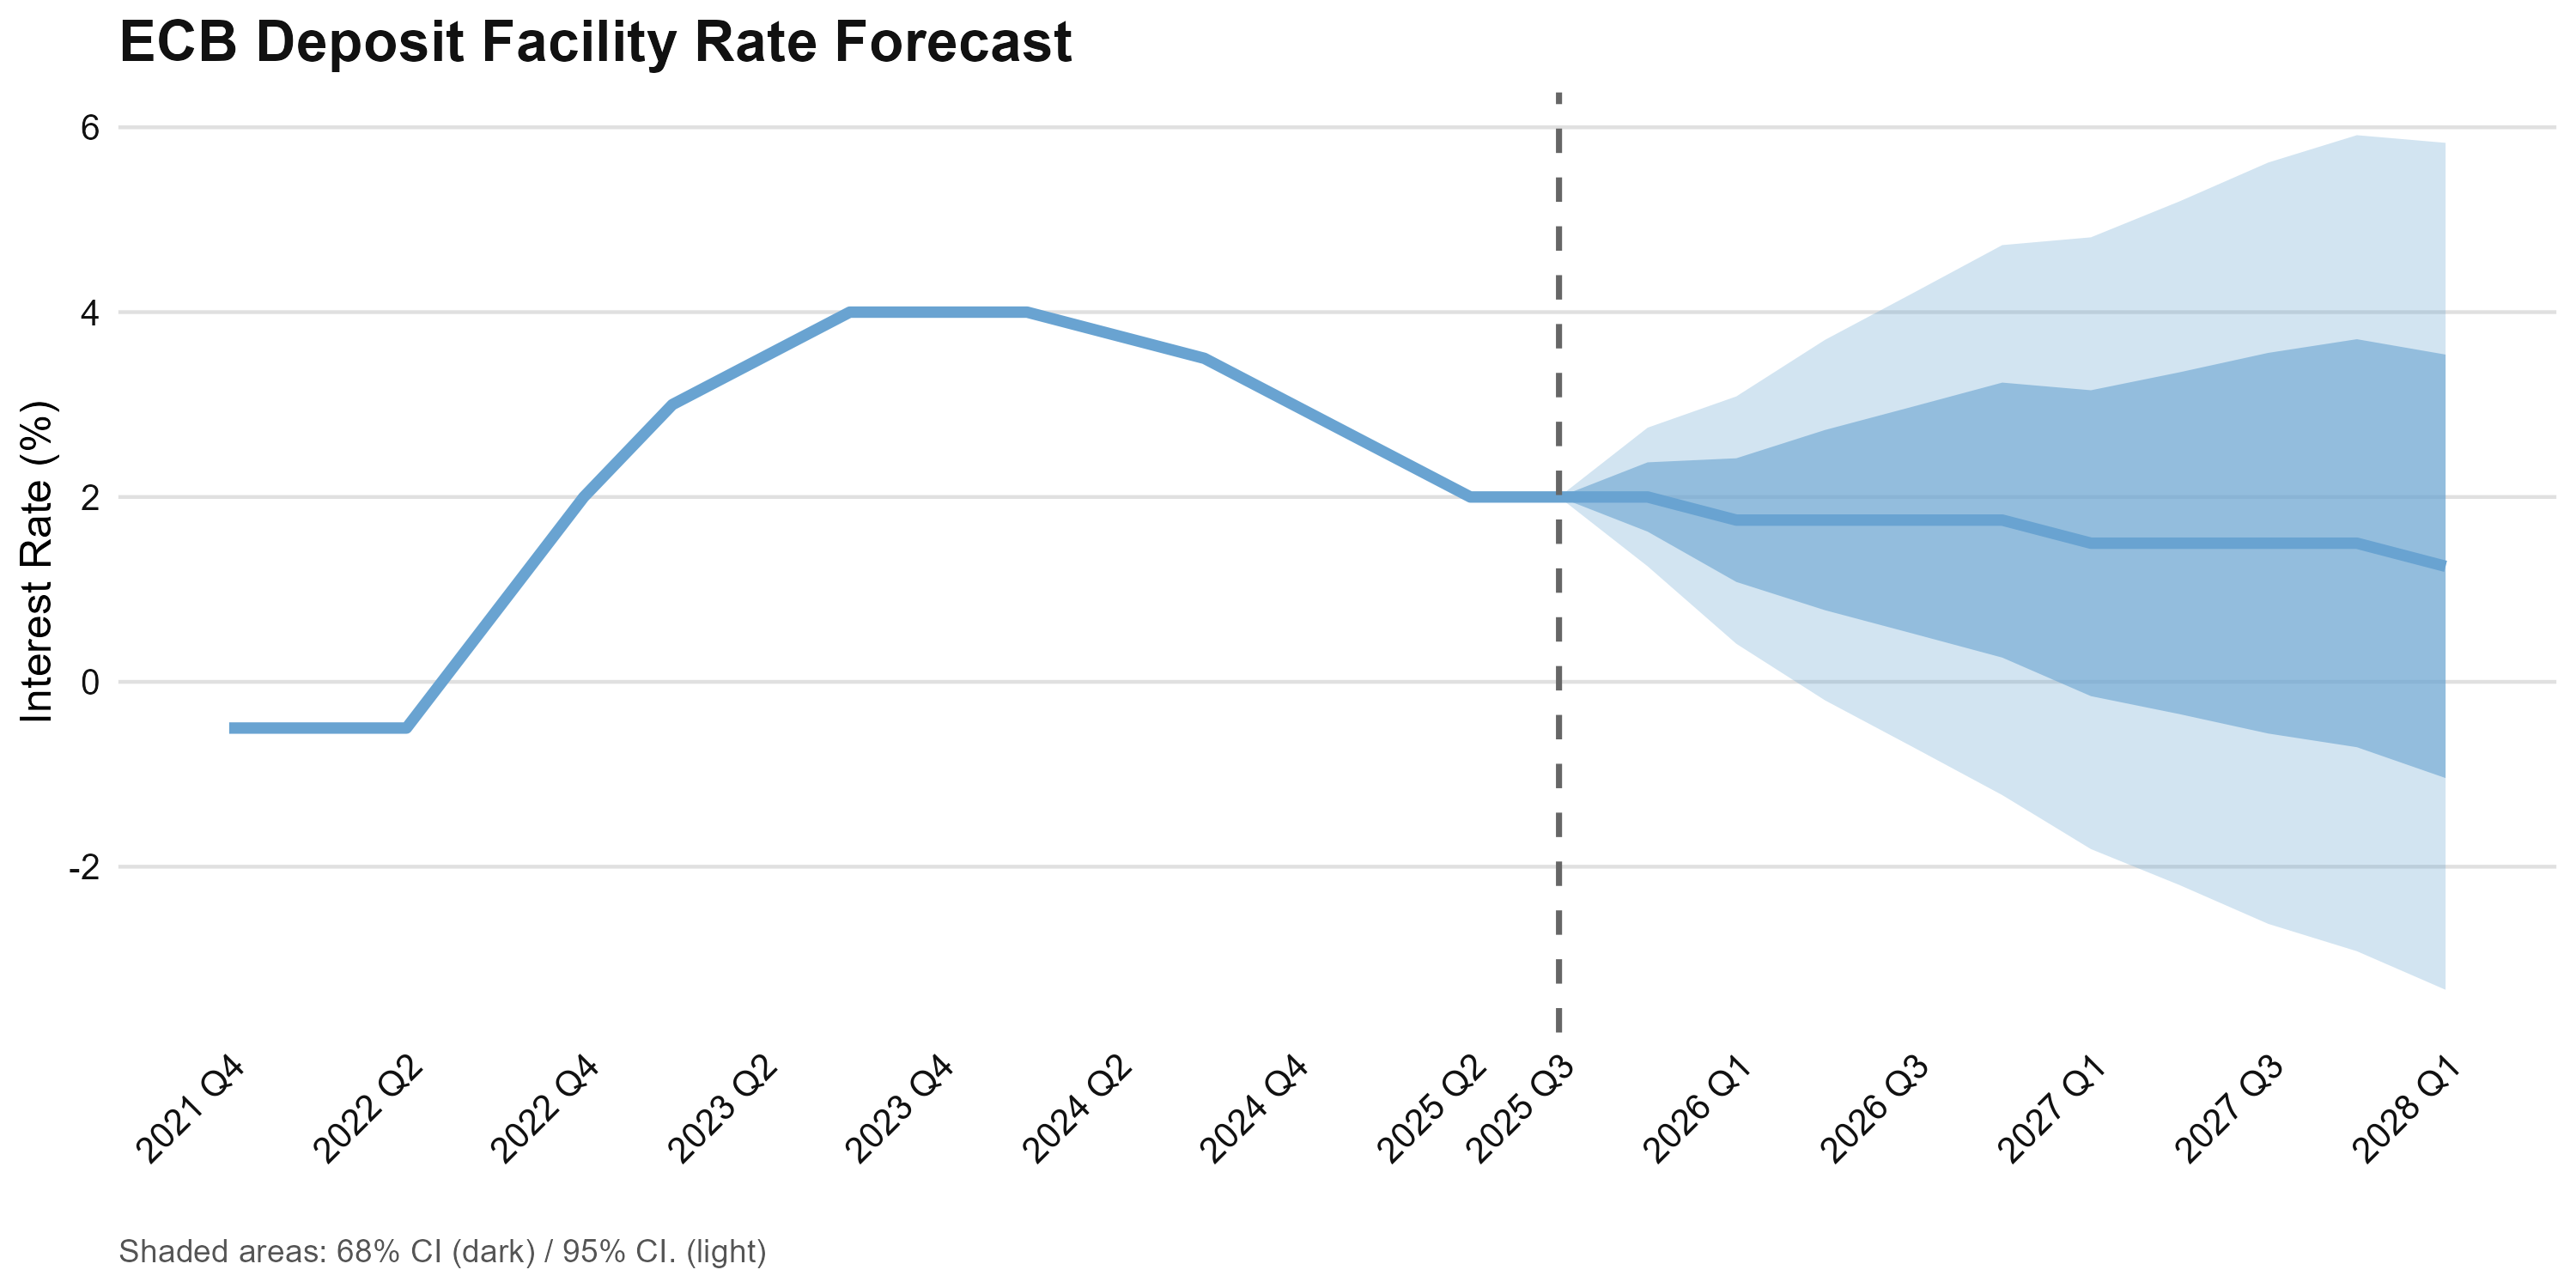
\includegraphics[width=\textwidth]{figures/forecast_plot.png}
        \caption[Forecast Results Plot]{Results for our forecast from 2025 Q4 to 2028 Q1}
        \label{fig:actual_forecast}
    \end{subfigure}
    \hfill % Adds flexible space between the images
    % Second Subfigure
    \begin{subfigure}[b]{0.48\textwidth}
        \centering
        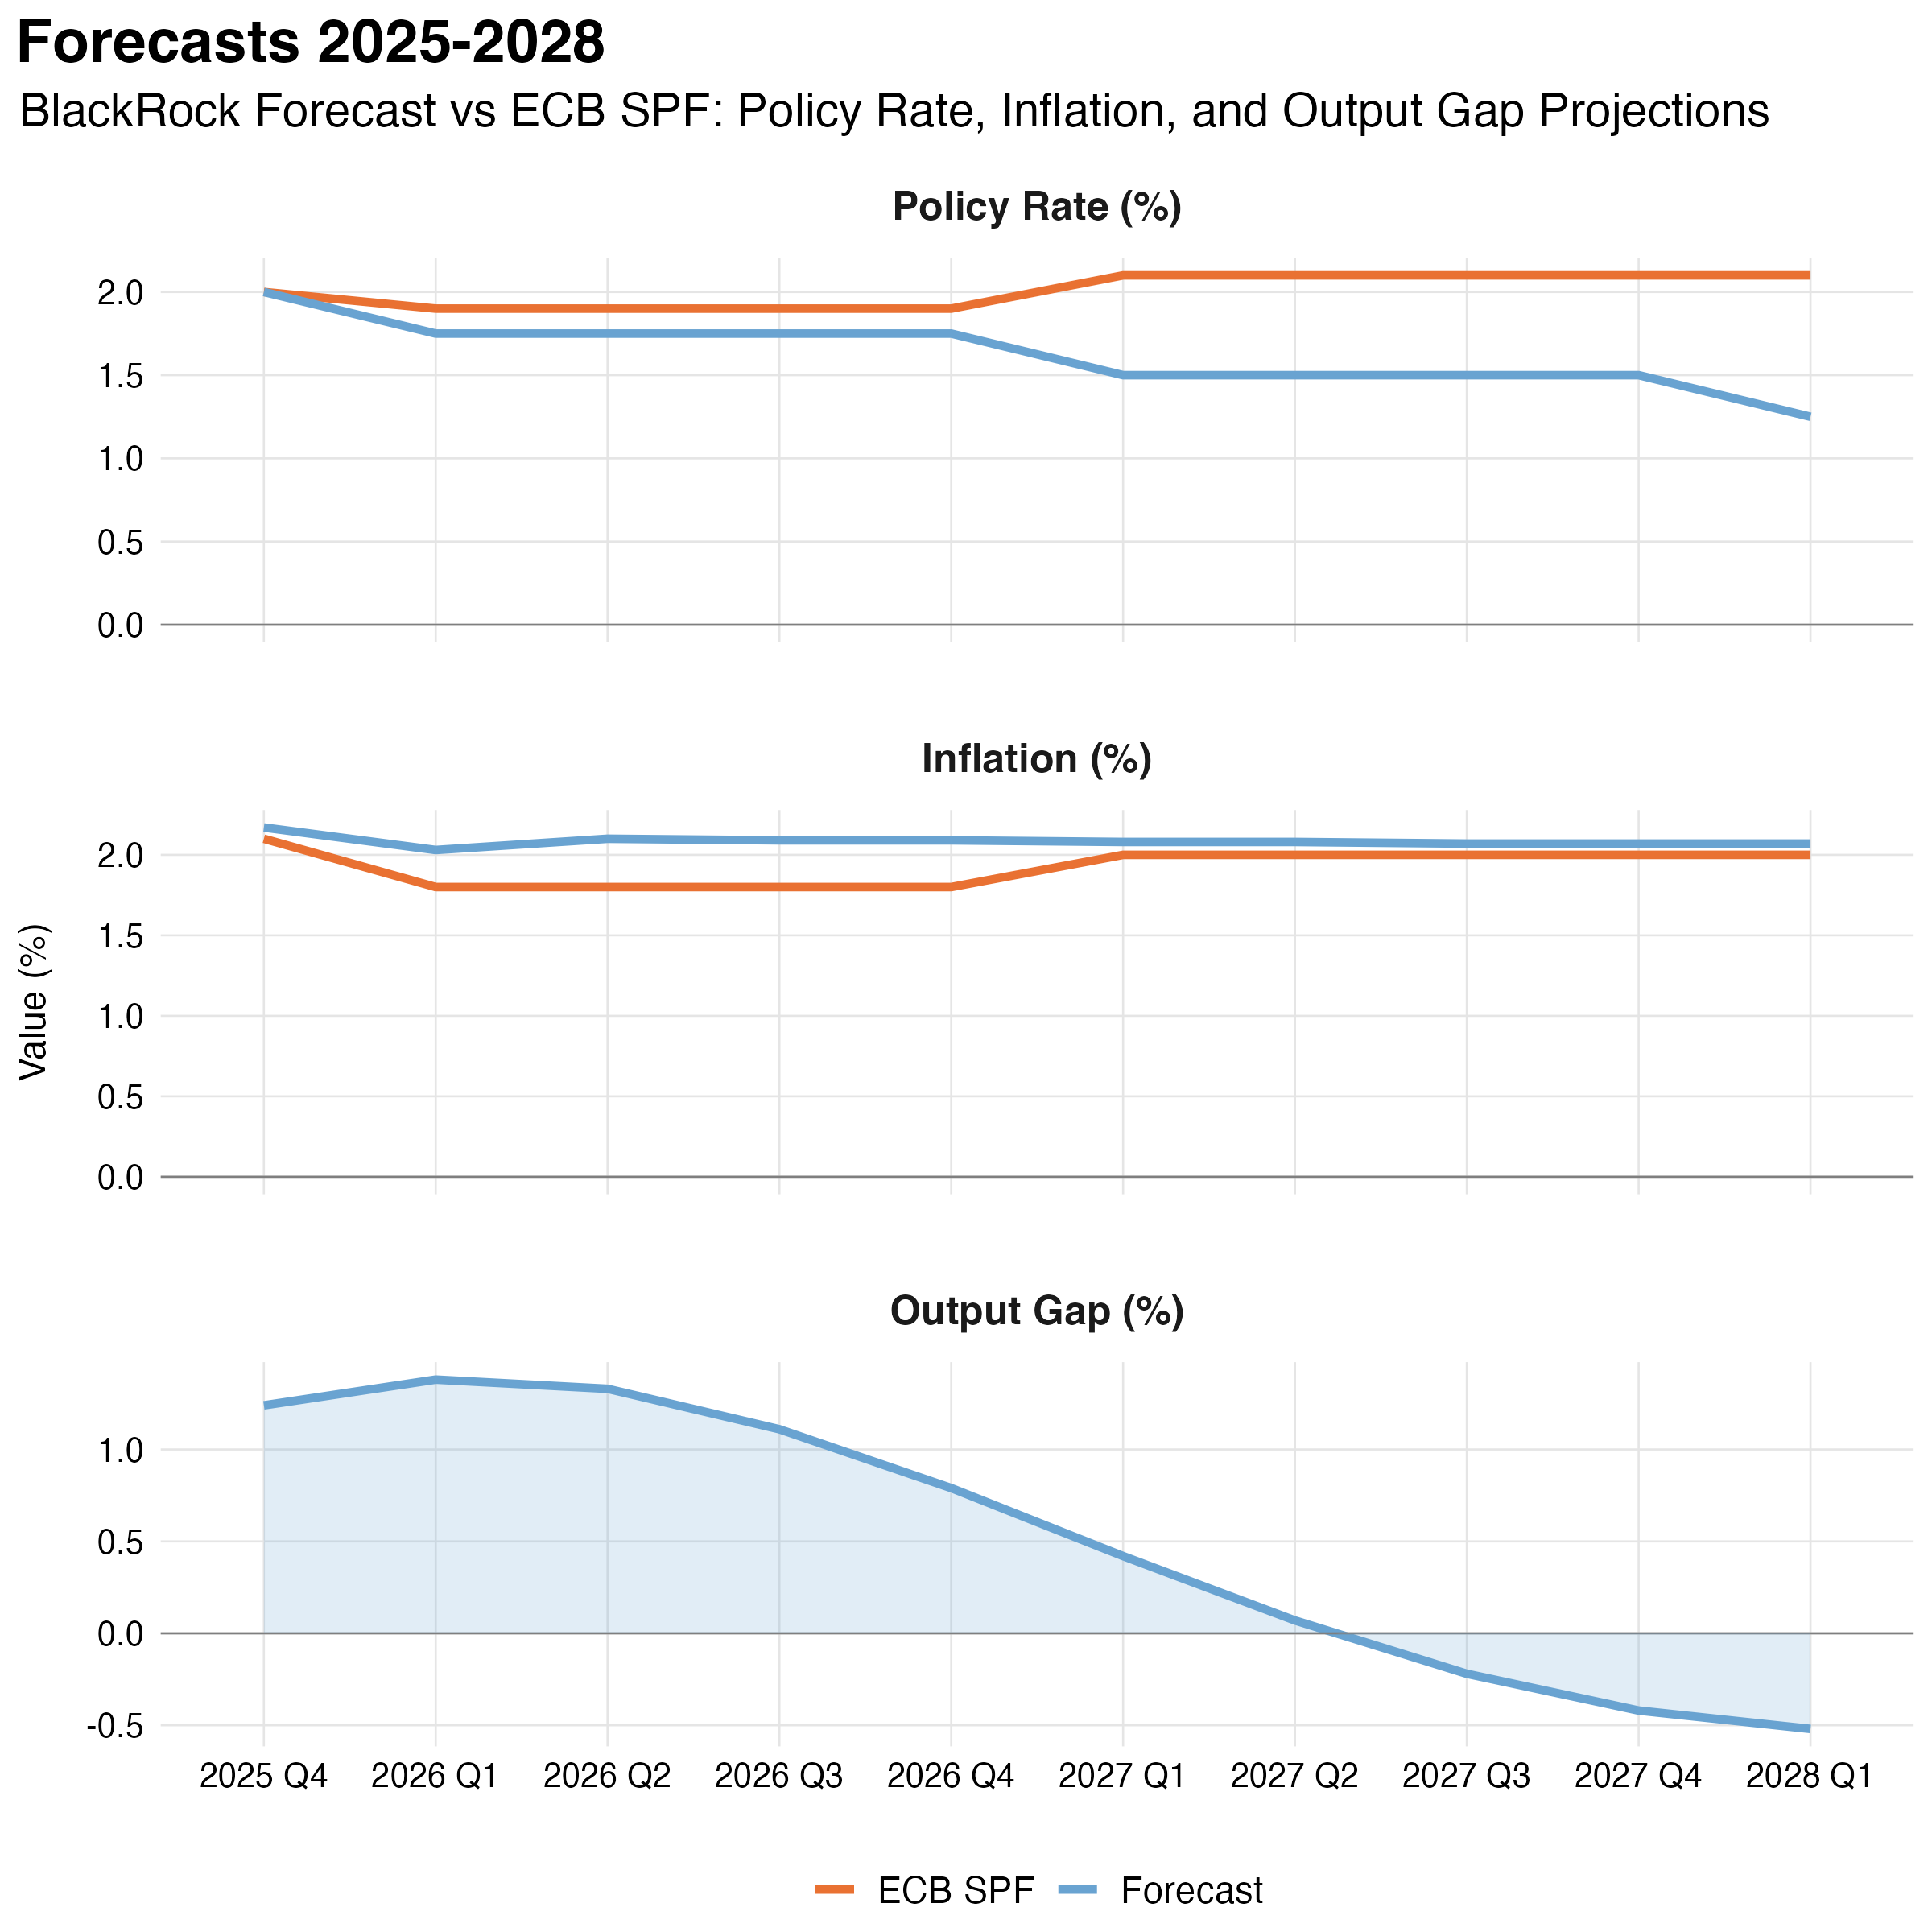
\includegraphics[width=\textwidth]{figures/forecasts_all_comparison.png}
        \caption[Forecast Comparison Plot]{Forecasts Comparison}
        \label{fig:forecast_comparison}
    \end{subfigure}
    \caption{Forecast Results \& Comparison}
    \label{fig:both_forecasts}
\end{figure}

\input{figures/stationarity_results}

\input{figures/Mincer_Zarnowitz_Test_Actual_Rate_with_Lag}

\input{figures/MSFE_Comparison_Trained_on_Actual_Rate_with_Lag}

\begin{figure}[h]
    \centering
    
\includegraphics[width=0.7\textwidth]{figures/spaghetti_errors_plot.png}
    \caption[Forecast Errors Spaghetti Plot]{Spaghetti plot of our forecast errors in evaluation sample, by horizon}
    \label{fig:spaghetti_errors}
\end{figure}

\begin{figure}[h]
    \centering
    % First Subfigure
    \begin{subfigure}[b]{0.48\textwidth}
        \centering
        
\includegraphics[width=\textwidth]{figures/densityridge_plot.png}
        \caption[Forecast Errors Density]{Distribution of our forecast errors}
        \label{fig:errors_density}
    \end{subfigure}
    \hfill % Adds flexible space between the images
    % Second Subfigure
    \begin{subfigure}[b]{0.48\textwidth}
        \centering
        
\includegraphics[width=\textwidth]{figures/FE_var_plot.png}
        \caption[Forecast Errors Variance]{Variance of our forecast errors, by horizon}
        \label{fig:errors_variance}
    \end{subfigure}
    \caption{Properties of Forecast Errors In Evaluation Sample}
    \label{fig:both_errors}
\end{figure}






\begin{comment}
\begin{figure}[h]
    \centering    
    \begin{subfigure}[b]{0.48\textwidth}
        \centering
        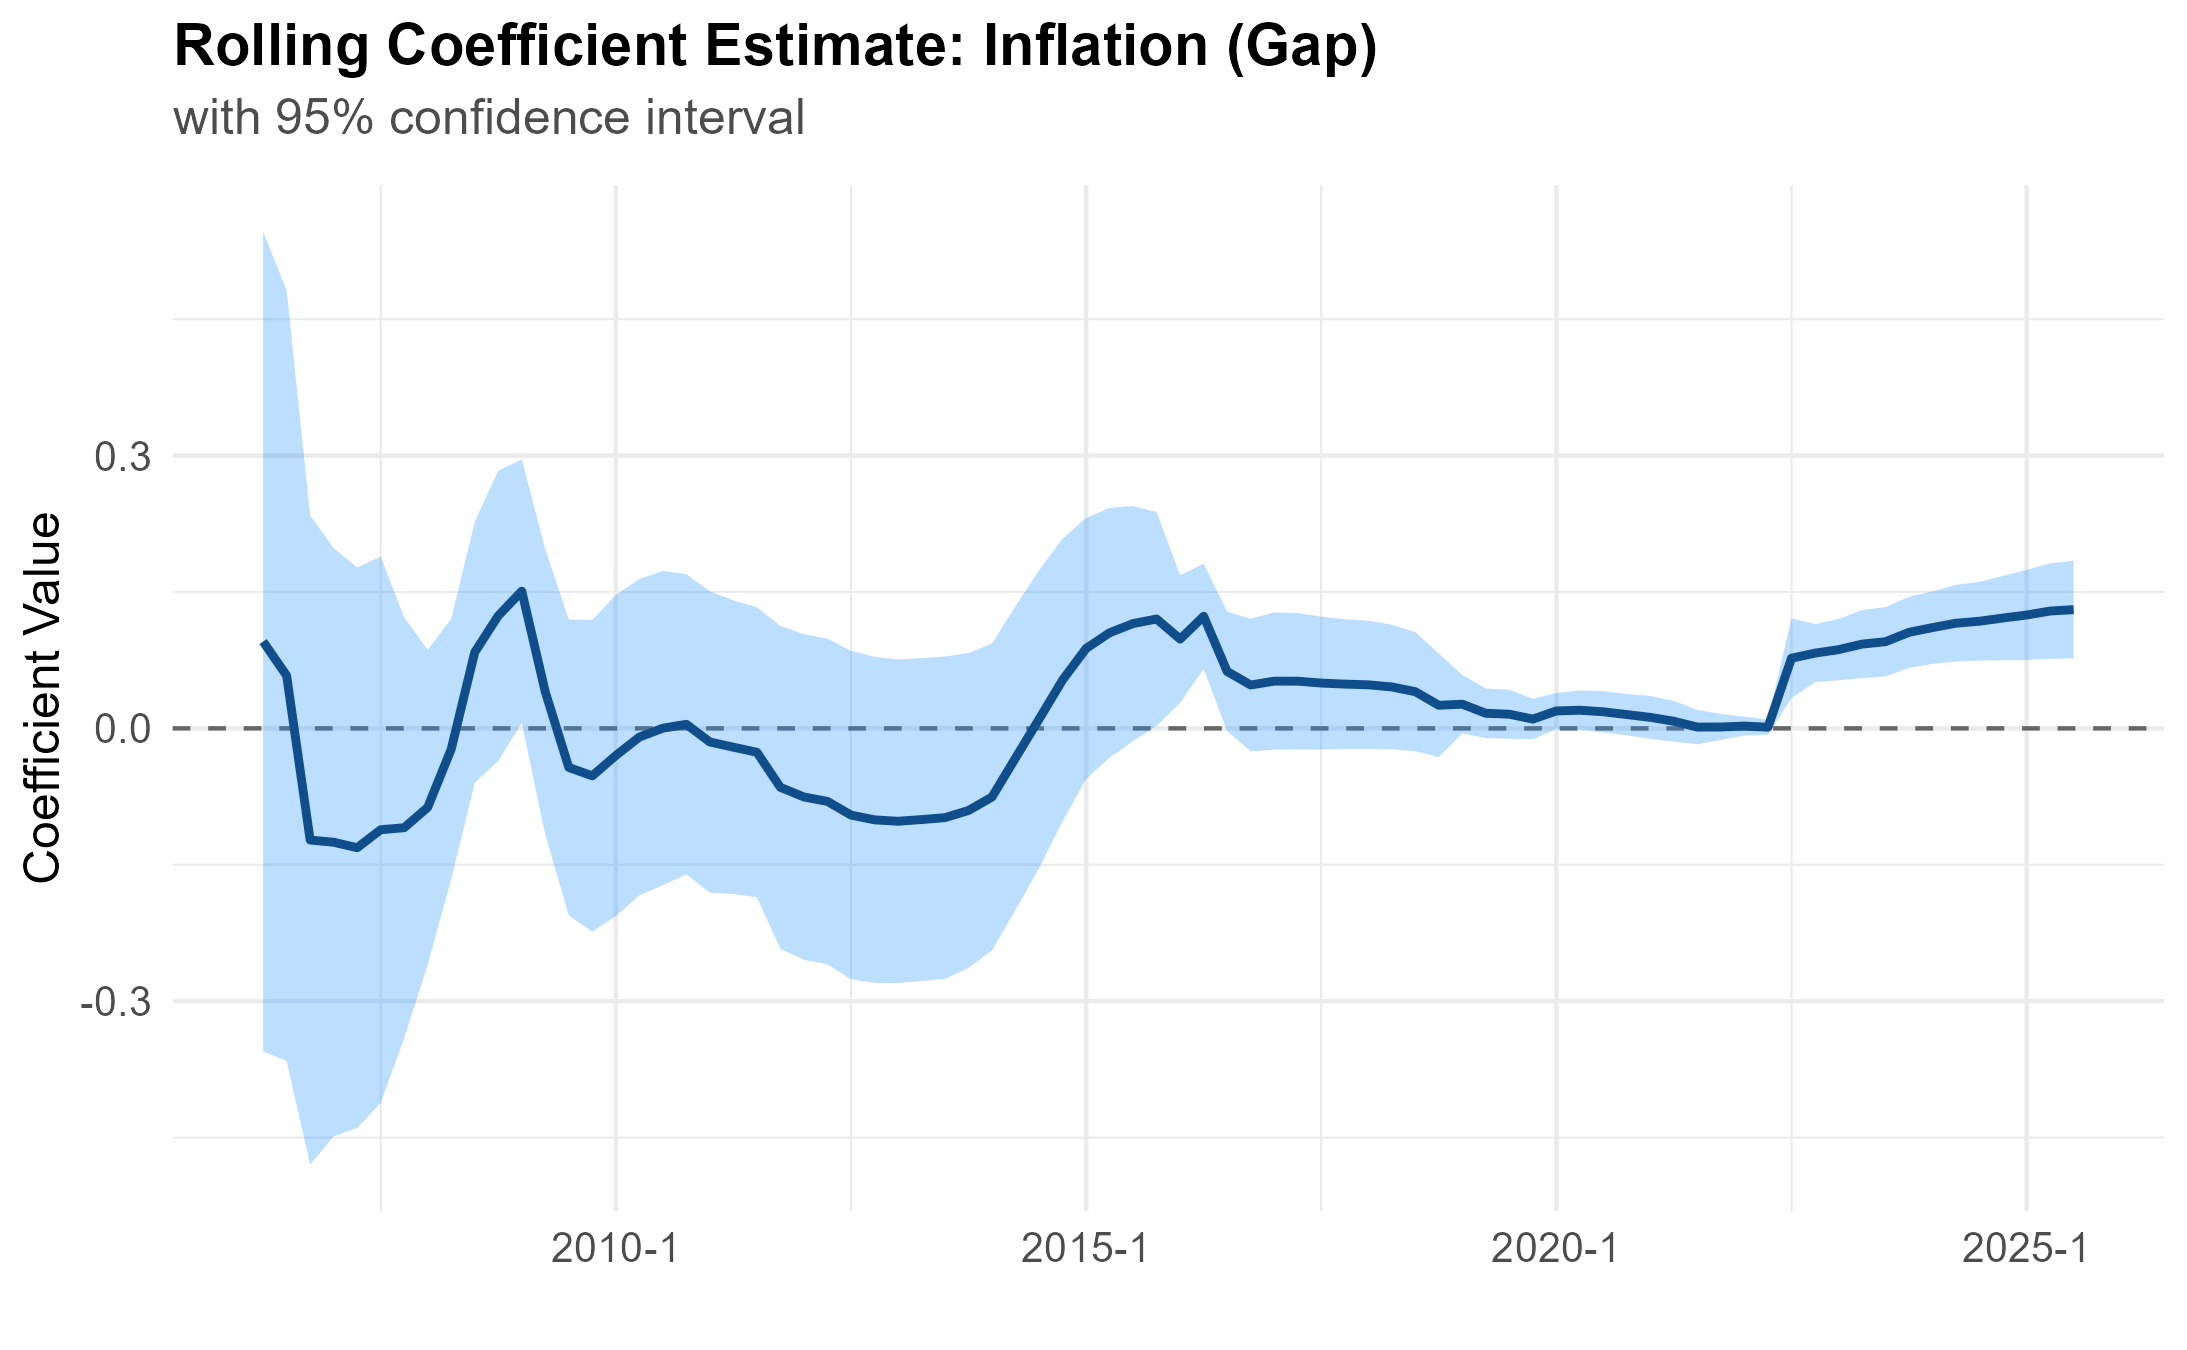
\includegraphics[width=\textwidth]{figures/roll_coef_Inflation (Gap).png}
        %\caption{Inflation Coefficient ($\beta$)}
        \label{fig:roll_TR_inf}
    \end{subfigure}
    \hfill % Adds flexible space between the images
    \begin{subfigure}[b]{0.48\textwidth}
        \centering
        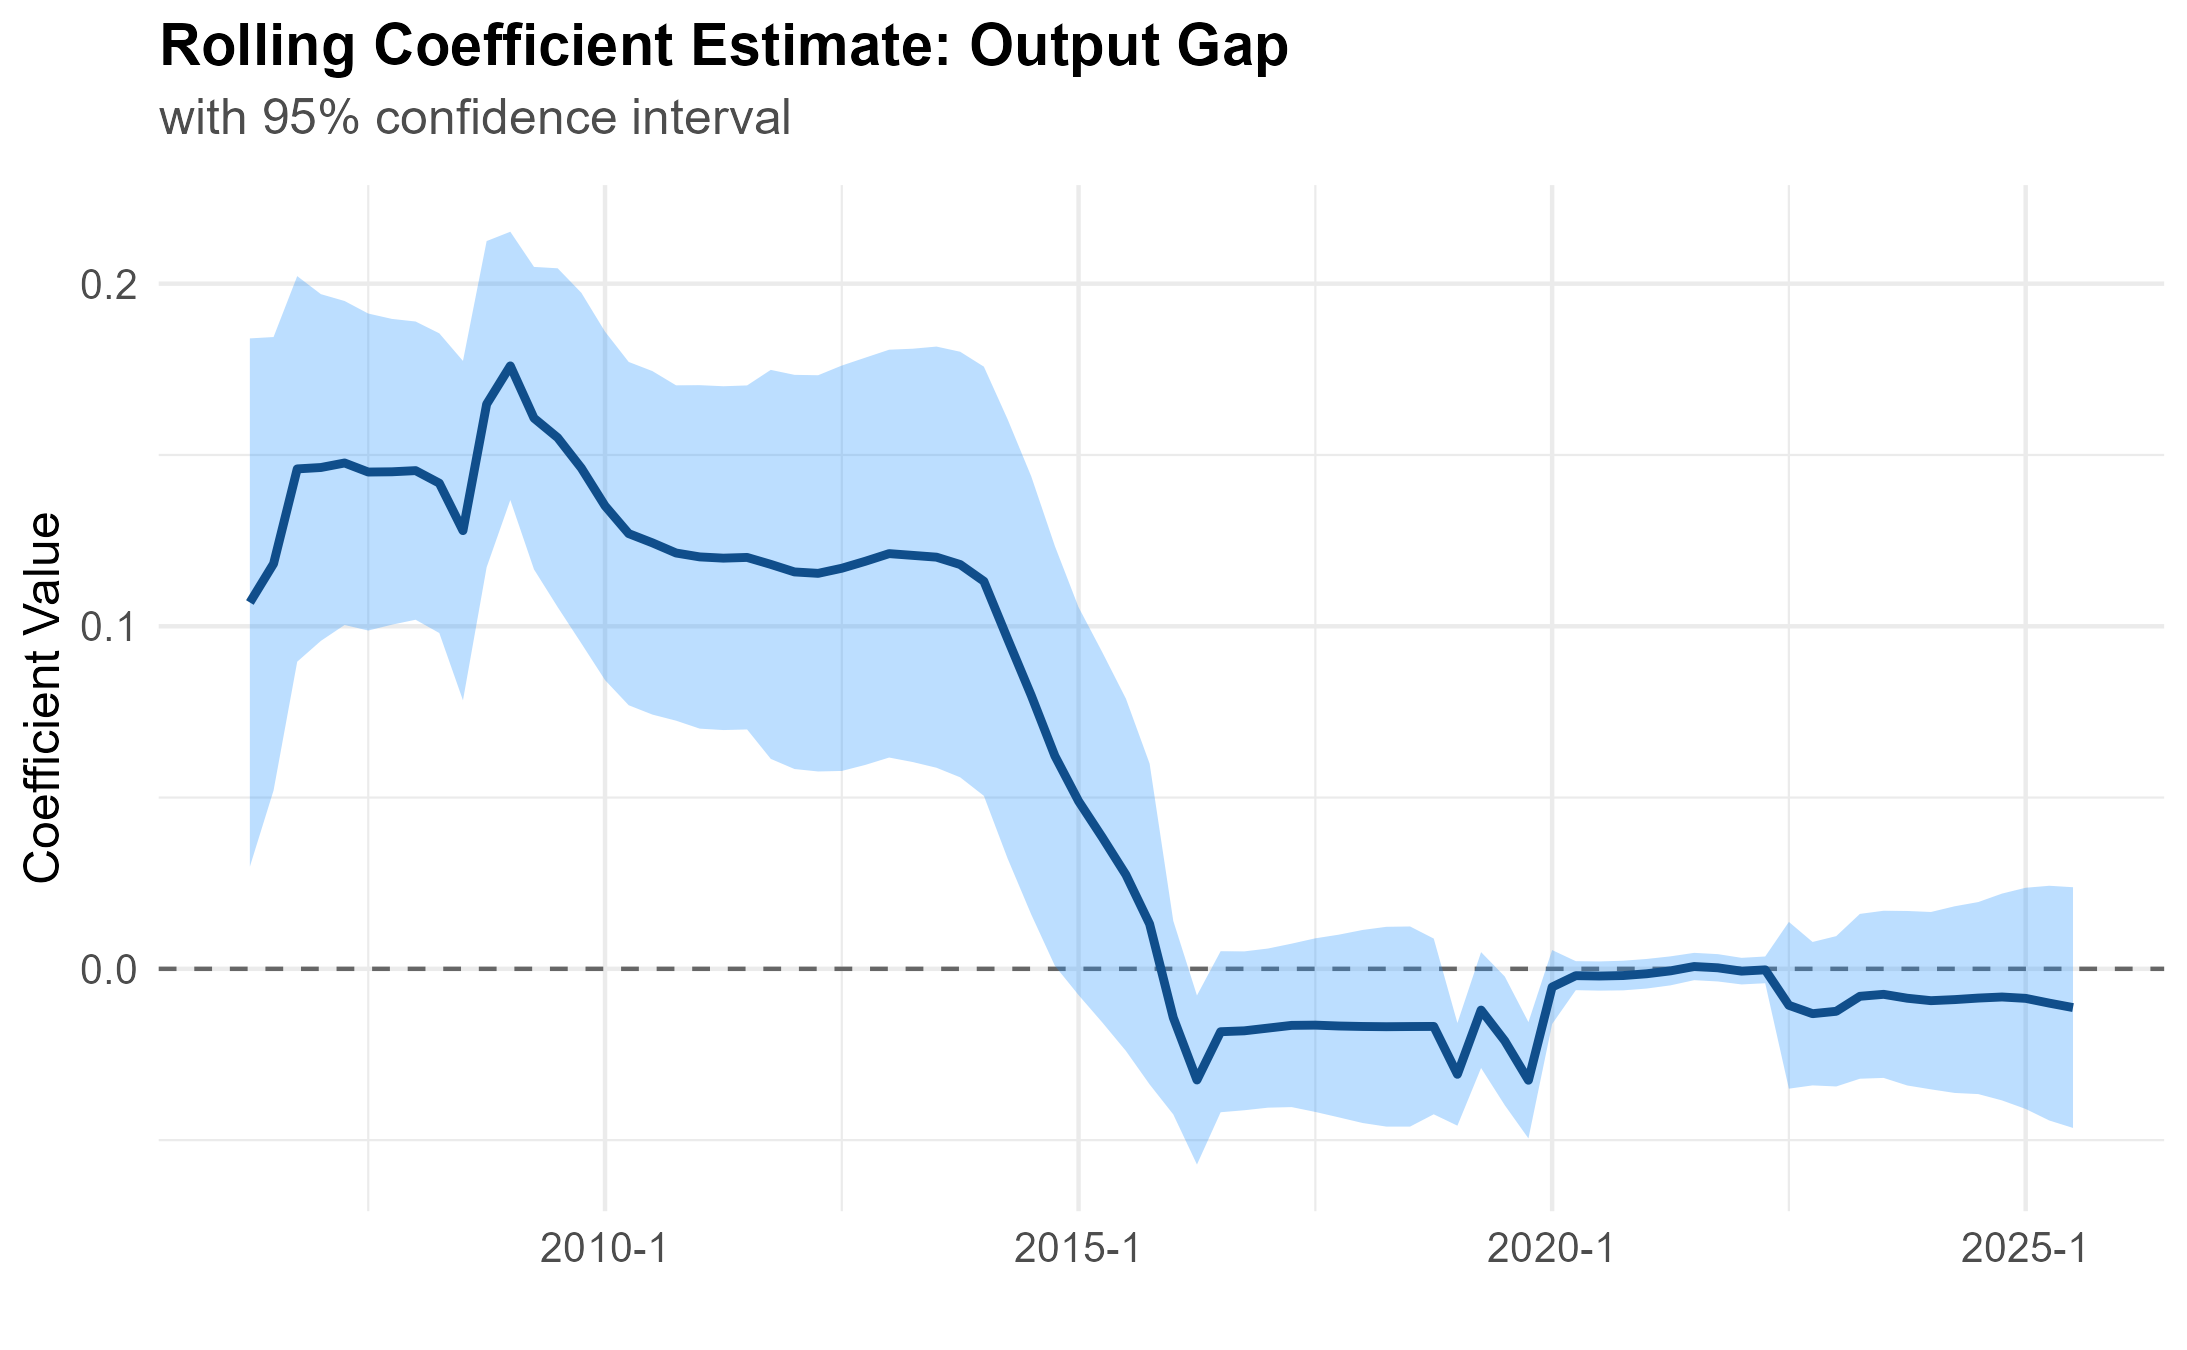
\includegraphics[width=\textwidth]{figures/roll_coef_Output Gap.png}
        %\caption{Output Coefficient ($\gamma$)}
        \label{fig:roll_TR_out}
    \end{subfigure}
    \hfill
    \begin{subfigure}[b]{0.48\textwidth}
        \centering
        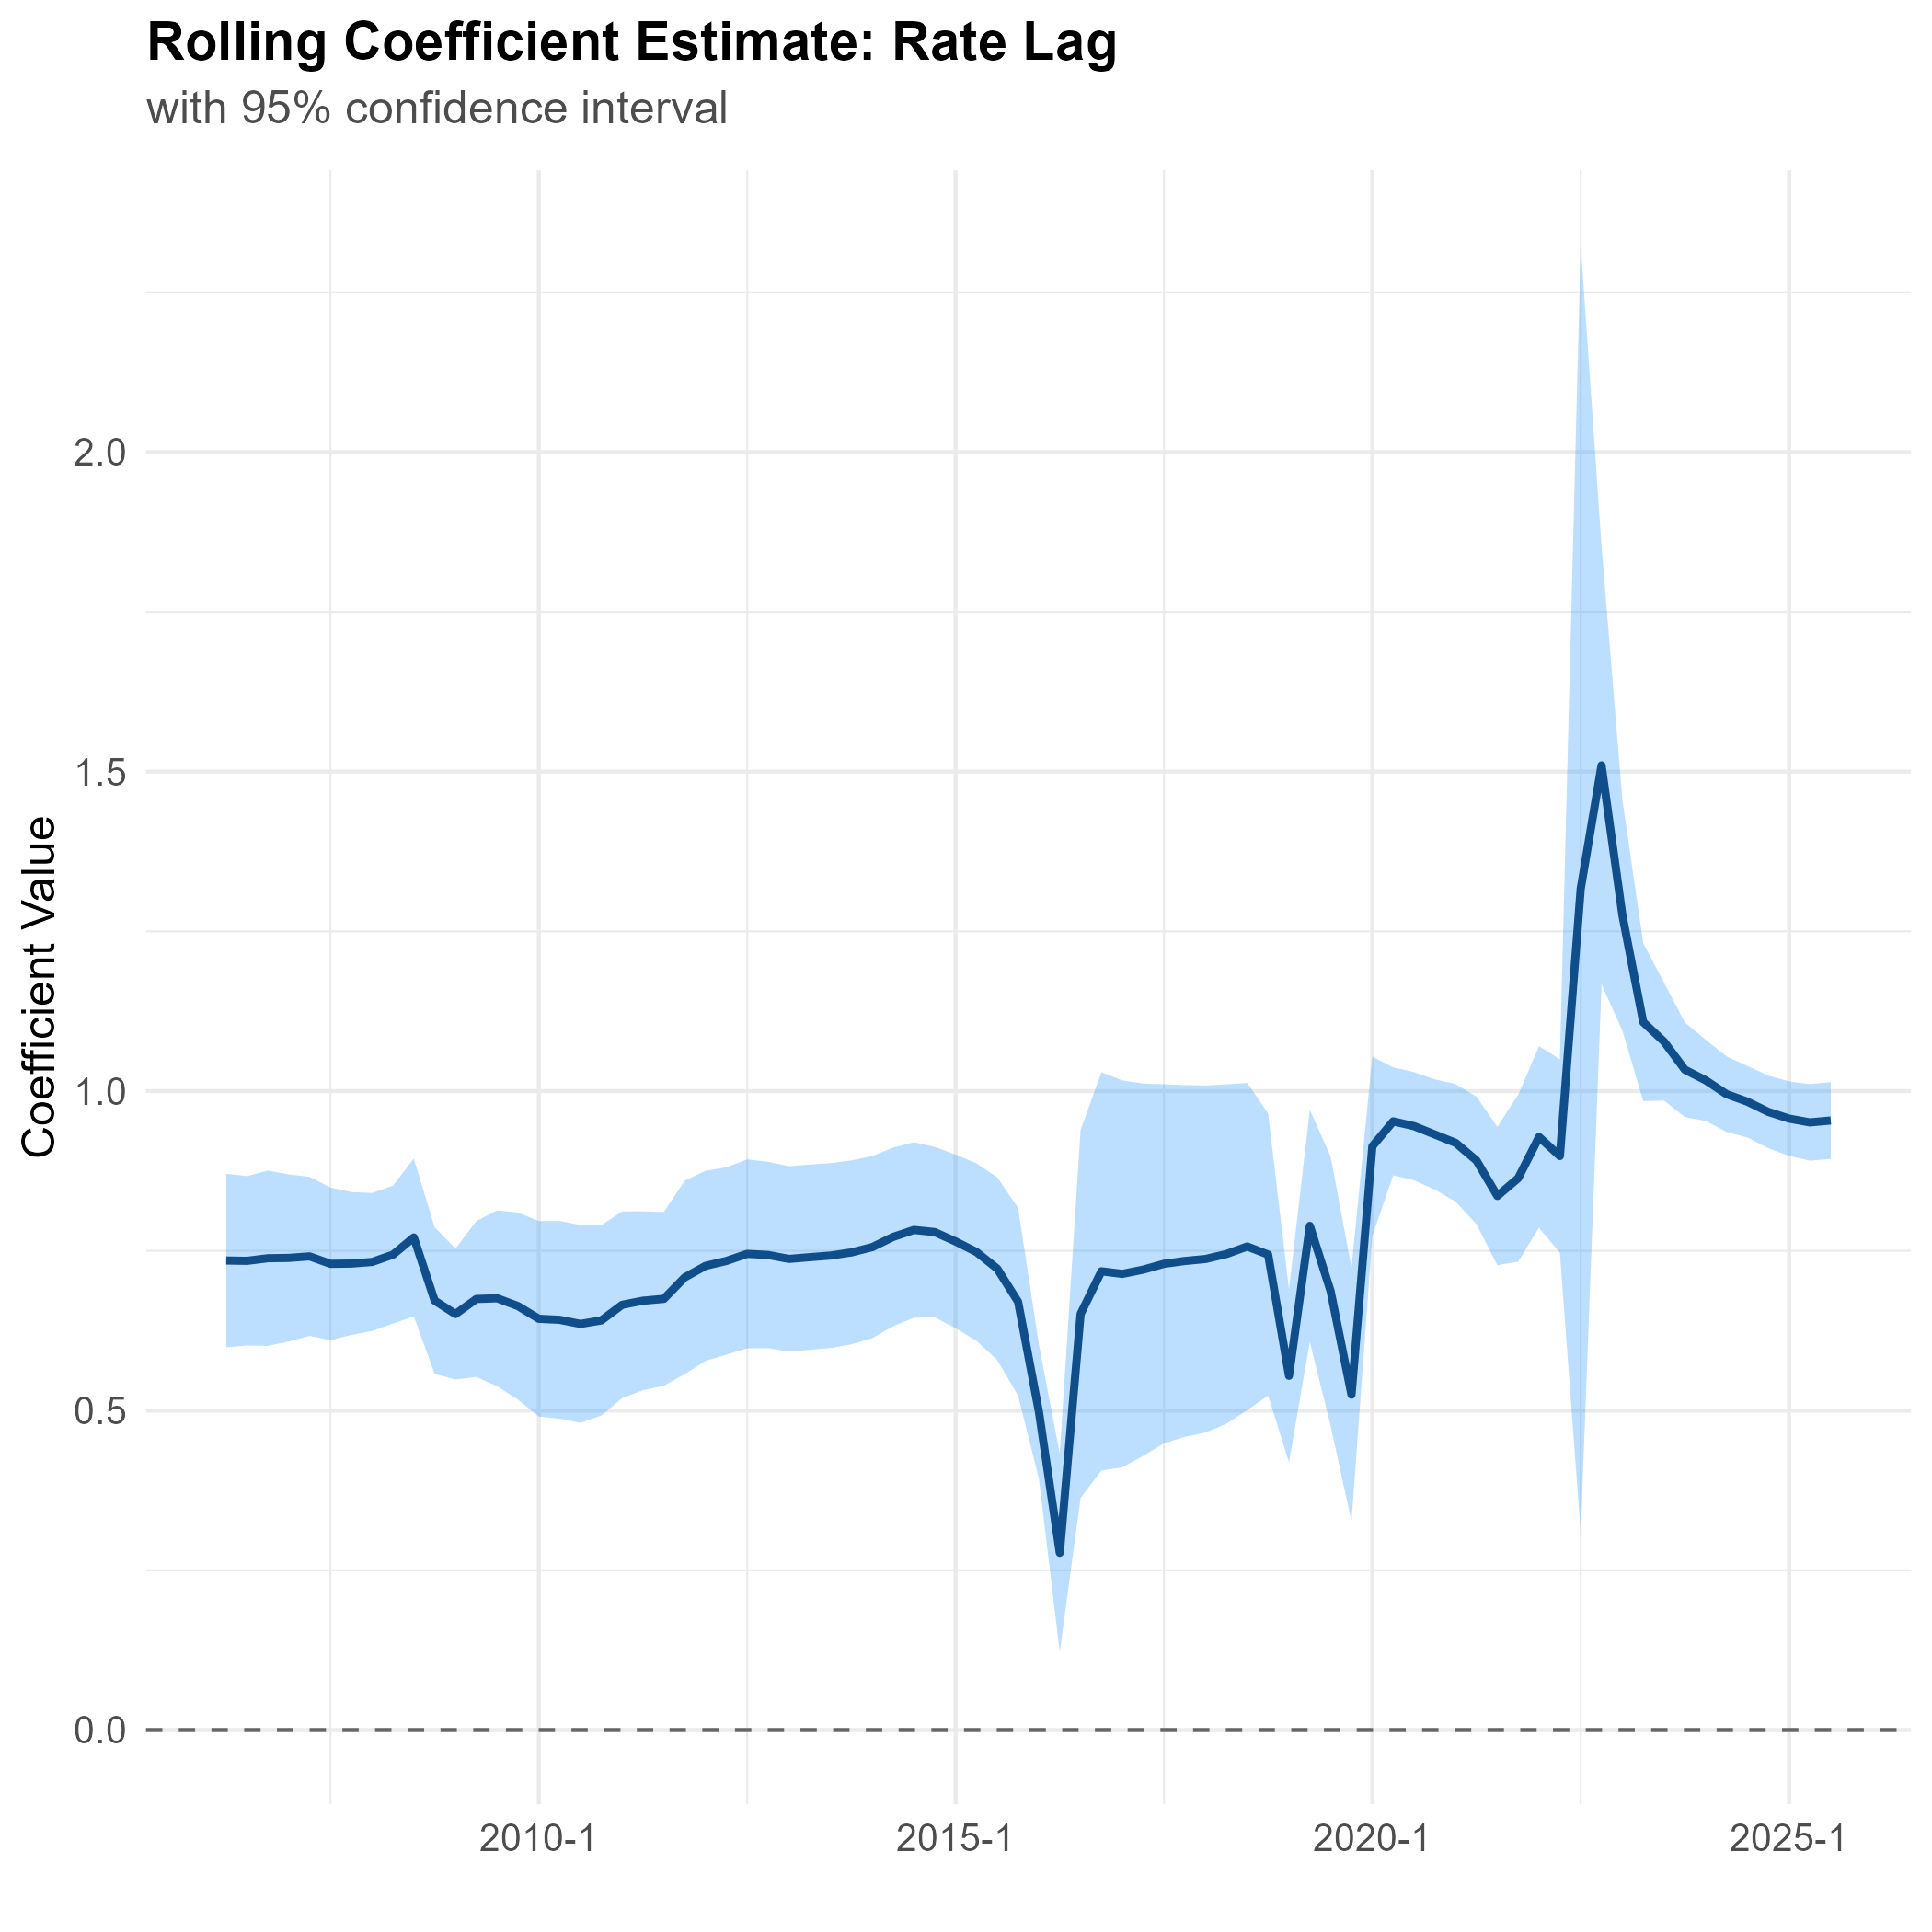
\includegraphics[width=\textwidth]{figures/roll_coef_Rate Lag.png}
        %\caption{Interest Rate Lag Coefficient ($\phi$)}
        \label{fig:roll_TR_lag}
    \end{subfigure}
    \caption{Rolling Taylor Rule Input Coefficients}
    \label{fig:all_TR_coefs}
\end{figure}
\end{comment}



\end{document}
